\chapter{SYSTEM ANALYSIS }
 
 \section{Module Description}
 The "Debug Defuse" game is divided into multiple functional modules, each playing a key role in ensuring smooth gameplay, real-time coding challenges, and an engaging user experience. The main modules include:
 \begin{itemize}
    \item \textbf{Player Movement Module:}This module is responsible for handling how the player moves within the 3D maze environment. It processes user inputs, such as pressing arrow keys or using a joystick, and translates them into smooth and responsive character movement. The module ensures that the player can navigate the maze without delays or glitches. Additionally, it includes collision detection, which prevents the player from walking through walls or objects, ensuring realistic interactions with the environment. The movement mechanics are designed to be fluid, avoiding jerky motions or unnatural behavior that could affect gameplay.
    \item \textbf{Checkpoint \& Challenge Module:}The maze is divided into multiple checkpoints, and this module ensures that when the player reaches a checkpoint, a coding challenge is triggered. The challenge appears as a coding question displayed on the screen, along with a text input field where players can type their solutions. This module ensures that the challenge mechanics function correctly, meaning the coding problem should only appear when the player reaches the designated checkpoint and should not disappear until it has been solved successfully.
    \item \textbf{Code Compilation \& Validation Module:}This module is crucial for evaluating the player’s submitted solutions. When a player enters code in the input field, the module sends the code to the JDoodle API, which compiles and executes it in real-time. The module then compares the output with predefined test cases to determine whether the solution is correct. If the code produces the expected results, the challenge is considered solved, and the player can move forward in the game. If the code is incorrect, the player must modify their solution and try again.
    \item \textbf{Game Progression Module:}This module controls how the game unlocks new areas based on the player’s performance. When a coding challenge is solved correctly, the module removes restrictions, allowing the player to continue exploring the maze. However, if the solution is incorrect, the module prevents further movement, forcing the player to retry the challenge until they succeed. This system ensures that players fully engage with coding problems before moving on, making it both a learning experience and a game mechanic.
    \item \textbf{UI \& Interaction Module:}The user interface plays a major role in the gaming experience. This module is responsible for designing and managing all UI elements, such as menus, coding input fields, game messages, and challenge prompts. It ensures that the interface is clear and easy to navigate, so players can focus on solving coding challenges without confusion. The module also displays error messages, compiler feedback, and any hints that might assist players in debugging their code. A well-designed UI improves engagement and ensures players enjoy the game while learning.
    \item \textbf{Feedback Module:}This module provides real-time feedback based on the player's coding submissions. When a player enters a solution, the system instantly notifies them whether it is correct or incorrect. If the answer is incorrect, the module highlights errors or provides hints to help the player debug their code. This feature is essential for maintaining player motivation, as it guides them in learning from their mistakes rather than feeling frustrated. By offering immediate feedback, players can correct errors and improve their coding skills more effectively.
    \item \textbf{Pause \& Resume Module:}The game allows players to pause and resume at any time without losing progress. This module ensures that when the game is paused, all ongoing actions—including player movement and coding challenges—are temporarily paused. Upon resuming, the game restores the previous state, allowing players to continue exactly where they left off. This is particularly useful in educational games, where players might need time to think through coding challenges before returning to gameplay.
    
\end{itemize}
\section{Business Rules}
Business rules are specific guidelines, conditions, or constraints that govern the operations of a
business or system. They define how processes and activities should be conducted to ensure
consistency, fairness, and alignment with business objectives. Business rules help ensure that the
system behaves as expected and meets the needs of users or stakeholders.\\\\
\textbf{Question Management}
\begin{itemize}
    \item All coding questions are stored in a structured JSON file to allow efficient retrieval and consistent formatting within the game.
    \item Only valid and complete questions are added to the JSON file. Each entry must include the question type, question text, description, sample input, and expected output.
    \item The game supports coding in four programming languages: \textbf{C, C++, Python, and JavaScript}, offering flexibility to players.
    \item Each submitted solution is validated by comparing the player's output against predefined test cases to ensure accuracy.
    \item During gameplay, questions fetched at each checkpoint are unique and do not repeat within the same game session.
\end{itemize}
\textbf{Gameplay Mechanics}
\begin{itemize}
    \item Players must solve coding challenges presented at each checkpoint within the maze to unlock the path forward.
    \item There is no time limit, but players cannot proceed unless the current challenge is successfully completed and passes all test cases.
    \item Each checkpoint activates a new coding question, and the game logic ensures the challenge must be solved to continue navigating the maze.
    \item Incorrect submissions prompt real-time feedback, encouraging players to revise and resubmit until the correct solution is provided.
\end{itemize}
\textbf{Code Submission and Validation}
\begin{itemize}
    \item Submitted code is compiled and executed in a secure environment using the JDoodle API, which supports multiple programming languages.
    \item For a solution to be considered correct, the output must match  predefined test case associated with the coding challenge.
    \item If the code fails to compile or passes the some test case, the player must remain at the current checkpoint and try again until the case is passed.
    \item The validation process is done in real-time, and players receive immediate feedback on the correctness of their solution.
\end{itemize}

\newpage
\section{Analysis of Architecture (and/ or) Algorithms}
{\large \textbf{Unity Game Engine}}\\\\
Unity is a powerful game development engine used for creating interactive 2D and 3D experiences. For Debug Defuse, Unity provides the foundation for smooth player movement, immersive maze navigation, and seamless integration of coding challenges, ensuring an engaging and dynamic gameplay experience.\\\\
\begin{enumerate}
    \item \textbf{3D Environment and Physics:}
    \begin{itemize}
        \item Unity’s 3D engine enables the creation of an interactive maze with realistic player movement and object interactions.
        \item Built-in physics ensures accurate collision detection for walls, platforms, and checkpoints.
    \end{itemize}
    \item \textbf{C\# Scripting and Game Logic:}
    \begin{itemize}
        \item Unity uses C\# to script core mechanics such as player movement, checkpoint activation, and UI interactions.
        \item State management allows smooth transitions between game states like movement, challenge activation, and game completion.
    \end{itemize}
    \item \textbf{Animation and UI Integration:}
    \begin{itemize}
        \item The Animator system helps create fluid animations for player movement and UI transitions.
        \item Unity’s UI tools enable intuitive interfaces for coding challenges,Start menu,Resume menu,feedback messages and level complete .
    \end{itemize}
    \item \textbf{API Integration and Debugging:}
    \begin{itemize}
        \item Unity easily integrates with external services like the JDoodle API for real-time code compilation and validation.
        \item Built-in debugging and testing tools help refine gameplay and fix issues efficiently.
    \end{itemize}
\end{enumerate}
\textbf{Why Unity for Debug Defuse?}\\\\
Unity provides a comprehensive game development framework that ensures smooth gameplay, interactive coding challenges, and an engaging experience for players. Its flexibility and real-time capabilities make it an ideal choice for developing Debug Defuse.
\section{Project Pipeline}
\begin{figure}[H]
    \centering
    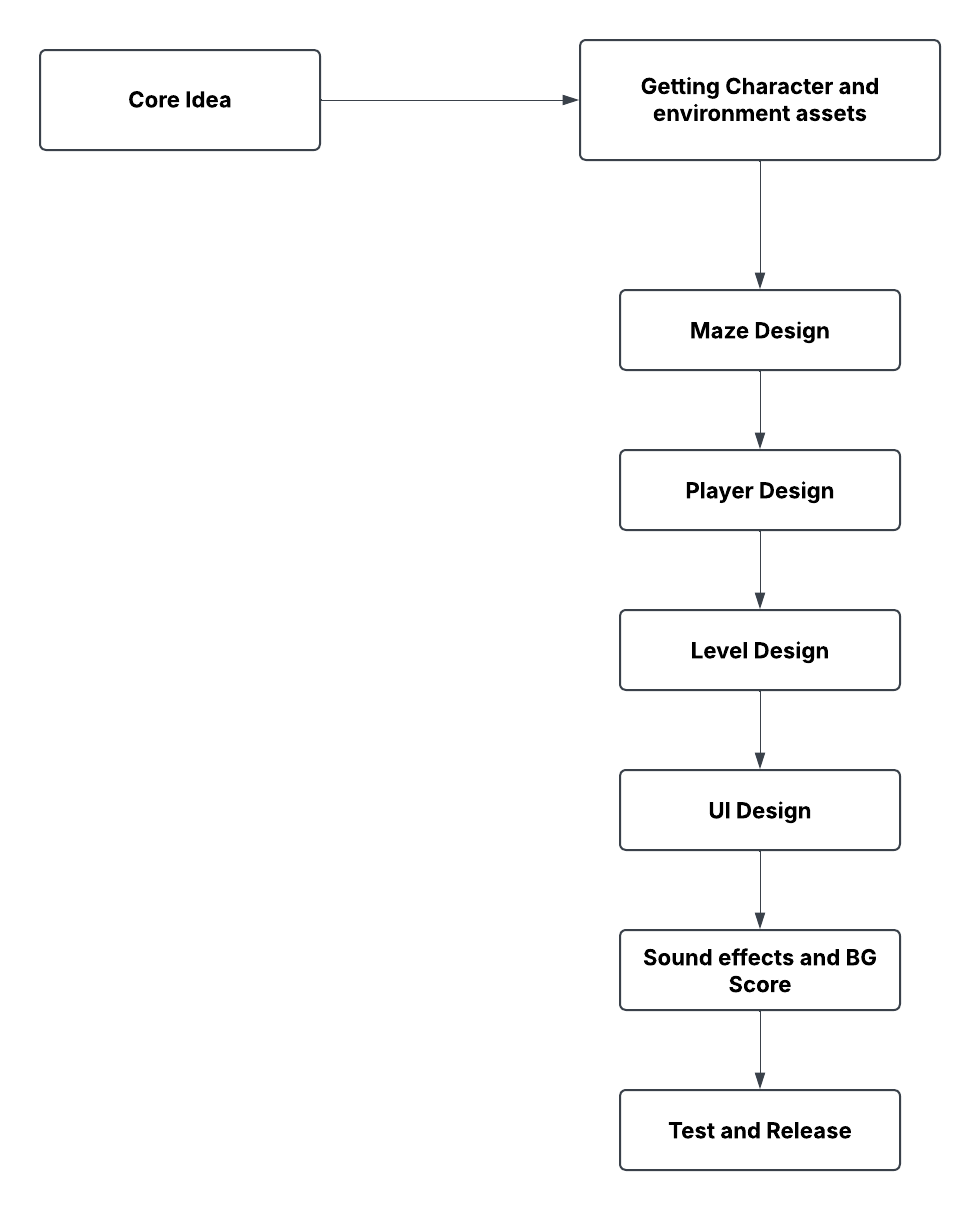
\includegraphics[width=1\textwidth]{project_pipe.png}
    \caption{Project Pipeline}
    \label{fig:Use_case}
\end{figure}

 \section{Feasibility Analysis}
 
 \subsection{Technical Feasibility}

 Technical feasibility assesses whether a project can be successfully developed and implemented using the current available technology, skills, and resources. It involves evaluating the tools, technologies, and infrastructure required for the project, along with the team's technical expertise.\\\\
 \noindent
The technologies chosen for the Debug Defuse project are highly feasible and align well with its requirements. The frontend utilizes the Unity game engine to provide an immersive and interactive interface, featuring animations, smooth character control, and a live text editor where players can enter their code directly within the game environment. For code compilation and testing, the project integrates the JDoodle API, which securely compiles and executes the player’s submitted code and validates it against predefined test cases in real-time. Coding questions and their corresponding test cases are managed using a JSON file, eliminating the need for a traditional database system. This approach simplifies data handling and makes the system lightweight and easy to maintain. Additionally, version control and collaboration are managed through Git and GitHub, ensuring streamlined development and teamwork. This combination of technologies ensures a scalable, efficient, and engaging gameplay experience, making it an excellent fit for the project’s objectives.

 
 \subsection{Economical Feasibility}
 Economic feasibility refers to the assessment of the financial aspects of a project to determine whether it is cost-effective and viable. It evaluates whether the benefits and potential returns of the project justify the costs associated with its development, deployment, and maintenance.\\\\
 The economic feasibility of the Debug Defuse project demonstrates that it is cost-effective and sustainable in both the short and long term. Development costs are minimized by utilizing free and open-source tools such as the Unity game engine (Personal or Student plan), which provides a powerful environment for building immersive gameplay and interactive coding interfaces. The coding challenges and test cases are managed using a simple JSON file, eliminating the need for complex and costly database systems. Code compilation and validation are handled through the JDoodle API, which offers a free tier suitable for small-scale usage, with flexible and affordable paid plans available if the project scales to handle more traffic. Ongoing maintenance costs are low, as updates and improvements primarily involve content updates to the JSON files and minor enhancements within the Unity project. This makes Debug Defuse a highly economical solution, ideal for both educational and entertainment purposes.


 
 \subsection{Operational Feasibility}
 Operational feasibility evaluates whether the project aligns with operational requirements and whether it can be smoothly integrated into existing processes.\\\\
 The operational feasibility of the Debug Defuse project evaluates how effectively the system can perform key functions such as fetching coding questions, validating player-submitted solutions, and providing real-time feedback. These features are designed to operate seamlessly through the integration of reliable technologies. The game is developed entirely in the Unity engine, which provides an engaging and responsive interface with immersive visuals, animations, and interactive gameplay elements. Coding challenges and test cases are managed through a structured JSON file, simplifying question management without the need for a complex backend or database system.\\\\
\noindent
Code compilation and validation are handled via the JDoodle API, which securely executes the player's submitted code and returns the results in real-time. This ensures an efficient and smooth coding experience, offering immediate feedback to players on their solutions. Features such as the live coding editor, instant error messages, and progression through checkpoints based on successful code validation make the system practical, intuitive, and user-friendly.\\\\
\noindent
Overall, Debug Defuse demonstrates strong operational feasibility. Its streamlined architecture, secure code execution via JDoodle, and user-centric design enable efficient functionality and a smooth gameplay experience. The system is adaptable for both individual learners and educational environments, reinforcing its potential to achieve its intended objectives.
 \section{System Environment}
 
 \subsection{Software Environment}
 \textbf{Unity Engine:}
 The core development of Debug Defuse is carried out using the Unity Game Engine, which provides a comprehensive platform for building interactive, immersive 2D and 3D games. Unity offers a powerful and flexible development environment, featuring a robust physics engine, integrated animation tools, and a highly customizable UI system. For Debug Defuse, Unity is used to create the 3D maze environment, manage player movement and interactions, and implement the user interface elements, including the live coding text input field, checkpoint interactions, start menu, pause/resume options, and game-over panels.\\\\
 \textbf{C\# In unity:}
 C\# plays a central role in the development of Debug Defuse, serving as the primary programming language for implementing game logic within the Unity engine. C\# scripts manage a wide range of functionalities, including player movement, collision detection with maze objects, checkpoint activation,camera manager and game state transitions such as starting, pausing, resuming, and triggering game-over conditions.
 \\\\
 \textbf{Mixamo(For Downloading Character Assets):}
 Mixamo is an online platform that provides free 3D character models and animations, making it easy to create realistic and animated characters for games. In my project, I used Mixamo to import a fully rigged character model with pre-made animations such as walking, running, and idle poses. This helped streamline the character development process, ensuring smooth and natural movements without the need for manual rigging or animation creation. Integrating Mixamo characters into Unity allowed for efficient character implementation, enhancing the visual appeal and immersive experience of the game.
\\\\
 \textbf{JDoodle:}
 The JDoodle API is a crucial component of the Debug Defuse game, providing real-time code compilation and execution functionality. JDoodle acts as an external online compiler that securely processes the code submitted by players during gameplay. When a player reaches a checkpoint within the maze, they are presented with a coding challenge, which they solve by entering code into a live text editor within the Unity interface. Upon submission, C\# scripts in Unity package the player's code and send it to the JDoodle API using HTTP POST requests.
\\\\
JDoodle compiles and runs the submitted code in a sandboxed environment, ensuring security and isolation. It then executes the code against predefined test cases to verify correctness. The API returns the compilation result, execution output, and any errors in real-time. Based on JDoodle's response, the game determines whether the player's solution is correct. If the code passes all test cases, the checkpoint is unlocked, allowing the player to continue navigating the maze. If the submission fails, the player is prompted to retry until the correct solution is provided.\\\\
\textbf{Sound and Music: Ableton Live}
The game’s sound effects and background music are composed using Ableton Live, a powerful digital audio workstation (DAW). Custom soundtracks enhance the game’s atmosphere,ensuring an immersive player experience.
 
 
 \subsection{Hardware Environment}
 \textbf{Processor (CPU):}i5 12th Gen\\\\
 \textbf{Memory (RAM):}16 GB\\\\
 \textbf{Storage:}512 GB SSD\\\\
 \textbf{Graphics Card (GPU):}RTX 3050 4 GB\\\\
 \textbf{Operating System:}Windows 11
 \newpage
 
 \section{Actors and roles}
 The system involves two primary actors: your actors.\\\\
\noindent
\textbf{Actors name:}
\\\\
 \textbf{Role:}
 \begin{itemize}

 \end{itemize}
\noindent
\textbf{Actors Name:}
\\\\
\textbf{Role:}
\begin{itemize}

\end{itemize}
 
 